\chapter{Proposed Model} 
\label{chapter:proposed_model}

%Population mobility modeling studies how populations are distributed and move through geographic space over time~\cite{brockmann2006scaling,gonzalez2008understanding}. Depending on the research question and available data, a model may cover spatial scales ranging from individual buildings and neighborhoods to cities, states, or countries, and temporal resolutions ranging from minutes to months or years. Rather than reconstructing every individual trajectory, population-level models describe the aggregate flows and state changes relevant to the phenomenon under study.
%SO: essa frase acima não tem muita cara de proposed, mas de intro. Não tá errado, só não precisaria.
%GA: comentei

%SO: abaixo, primeira vez que se fala em loduspop?
%GA: vou adicionar na intro, mas mantive aqui também
In this work, we propose LODUS, a flexible framework for population simulation in which heterogeneous populations are represented as variable-sized groups called \textit{blobs}. Blobs can move between locations, change their characteristics, and split or merge as different subsets of the population are affected. This representation allows the simulation resolution to be adapted to the available data and experiment requirements without requiring every person to be modeled as an independent agent. The proposed framework consolidates the environment-oriented representation introduced in LODUS~\cite{silva2020lodus} with the population-simulation mechanisms later developed in LodusPop~\cite{silva2026lodusPop}. %LodusPop é parte do LODUS %SO: incluir ref
%GA: Added



The framework separates the structures and rules shared by all simulations from behavior specific to an application domain. Its core model comprises three closely related elements: an environment containing regions and points of interest; a population represented by blobs and population templates; and an ordered system of routines and actions that changes the simulation state. 
A fourth element, the plugin layer, configures and extends this core with domain-specific population characteristics, location attributes, routines, action types, simulation-step updates, observations, and output recording. This separation allows the same population representation and simulation mechanisms to be reused across different application domains.

LODUS can be configured using real-world, derived, or synthetic data. %SO: abaixo são exemplos, certo? Então deixa claro
%GA: sim, ajustei o paragrafo
Figure~\ref{fig:data_diagram} illustrates examples of data sources that can be used to construct and configure a simulation. Geographic data, such as GIS datasets or OpenStreetMap, may define regions, points of interest, their types, and their attributes. Census or synthetic-population data may define the initial distribution and characteristics of the population, while Origin--Destination matrices, GPS observations, surveys, or programmed inputs may provide mobility information and parameters for population behavior. 
Experiment configurations select the plugins used in a simulation and define their parameters. These sources are illustrative rather than required: other datasets can be incorporated provided that they can be transformed into the information required by the model or its domain-specific extensions.


%SO: esse Data Sources são exemplos né? Se sim, eu deixaria claro que outros podem ser plugados. Gostei muito da figura
\begin{figure}[ht]
 \centering
 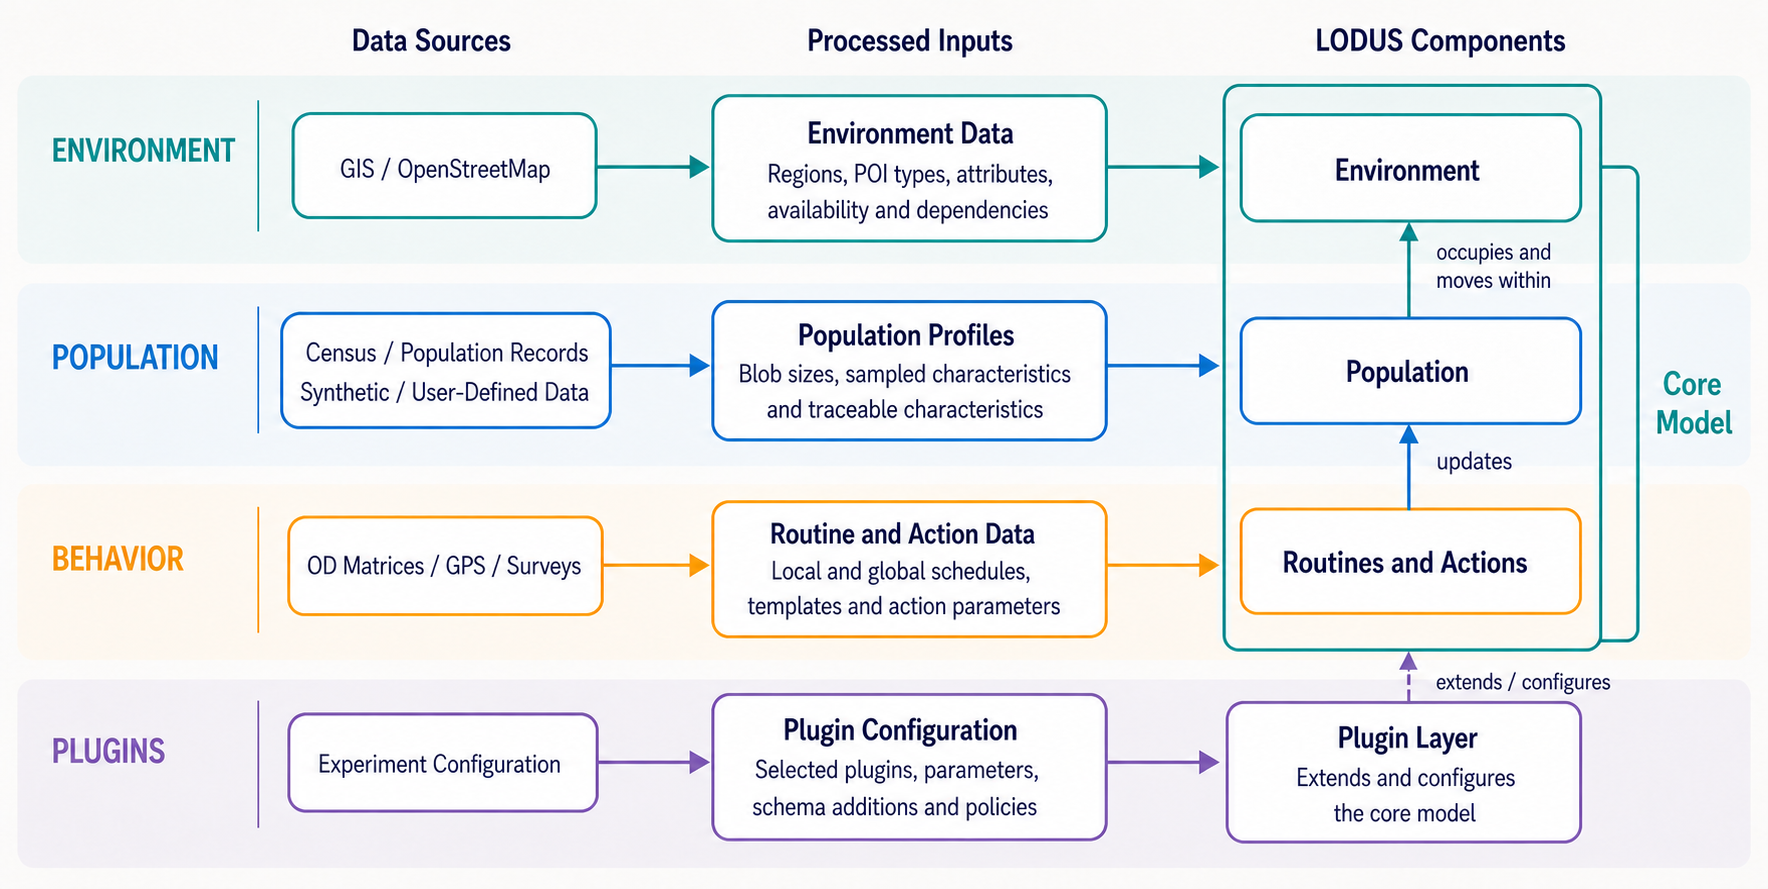
\includegraphics[width=0.98\textwidth]{fig/model/DataDiagramAlternativeCrop.png}
 \caption{Integration of example data sources into LODUS. Geographic, population, mobility, synthetic, and experiment-configuration data are transformed into environment data, population profiles, routine and action definitions, and plugin configurations. These inputs initialize the environment, population, and routines and actions of the core model, while plugins configure and extend the domain-specific characteristics and behavior considered in each experiment.}
 \label{fig:data_diagram}
\end{figure}

%SO: acho que os próximos 3 parágrafos são sobre a fig, né? Eu colocaria itens para ficaar fácil de ver que são sobre as partes da fig
%The population representation draws on aggregation strategies used in macroscopic crowd and mobility models~\cite{thalmann2007crowd,treuille2006continuum}. A LodusPop blob is conceptually related to abstractions such as clouds and legions~\cite{antonitsch2019bioclouds}, but is designed to represent larger and potentially heterogeneous populations. Sampled characteristics retain distributions within a blob, whereas traceable characteristics identify properties shared by its entire population. Population templates can select a subset of a blob according to these characteristics, allowing an action to affect only the relevant population and causing the blob to split when necessary.

%The environment design builds upon the approach introduced by Silva et al.~\cite{silva2020lodus}, while removing dependence on a fixed geographic hierarchy. Regions and points of interest can represent entities at the spatial resolution required by an experiment. Points of interest also have semantic types, extensible attribute mappings, local routines, direct availability conditions, and dependency constraints. They therefore represent not only places occupied by the population, but also the location state and demand that drive simulation behavior.

%This design supports the inversion of responsibility that characterizes LodusPop. Instead of requiring every individual or population group to independently choose a destination, points of interest use routines to request populations with particular profiles. For example, a school may request children during a given period, while a hospital may request patients satisfying a health-state predicate. If a requested location becomes unavailable, the core environment records that condition, while a plugin determines whether the corresponding demand is suppressed, queued, redirected, or otherwise adapted. Domain policies consequently remain explicit extensions rather than implicit properties of the population model.

%SO: ent~~ao :) os items estão abaixo.... será que precisa do texto acima, itens abaixo e mais as subsections abaixo? gosto dos itens e subsections. Não sei se o texto acima é necessário. Se fores tirar, lembra de comentar que a figura representa blabla e será detalhada a seguir. Daí tira esse "remainder" abaixo e já cola com as proximas subsectyions
% GA: comentei acima e resumi
The model is organized into four elements, detailed in the following sections:

\begin{itemize} 
    \item the \textit{environment}, represented by regions and typed points of interest with attributes, local routines, population contents, availability conditions, and dependency constraints; 
    \item the \textit{population}, represented by blobs, sampled and traceable characteristics, population templates, and split and merge operations; 
    \item \textit{routines and actions}, which provide an ordered mechanism for selecting populations and changing the simulation state; and 
    \item \textit{plugins}, which configure and extend the core model with domain-specific characteristics, location attributes, routines, action types, simulation-step updates, observations, and outputs. 
\end{itemize}


\section{Environment}
\label{sec:environment}

To adapt our population mobility simulation to different spatial scopes, we model the environment as an abstract graph composed of \textit{regions} and \textit{points of interest}. The regions ($R$) represent areas of physical space in the virtual world that can contain points of interest ($P$), which represent locations that motivate human travel and that can have population groups (i.e., blobs $B$).
When setting up a simulation, users define the spatial scope that $R$ and $P$ represent. For example, in a city simulation, $R$ could correspond to districts, while $P$ might represent markets, malls, hospitals, residential buildings, and commercial centers.


A region $R$ is represented as a finite set of points of interest $\{P_1,\ldots,P_m\}$. Each point of interest combines a semantic description of the location, its current population, its local behavior, and its availability conditions. We represent $P_i$ as

\begin{equation}
P_i=\bigl(\tau_i,\bm{\alpha}_i,\bm{B}_{P_i},\bm{Ro}_{P_i},\bm{C_i}(t),D_i\bigr),
\label{eq:poi_definition}
\end{equation}

All the parameters are detailed next. %Talvez colar no próximo paragrafo?

%SO: abaixo achei sucinto, type of what? attribute mapping to what??? é a primeira vez que o leitor lê isso, então tem que dar um pouco mais de info.... OU logo abaixo dessa frase tu faz como no exemplo abaixo
%where $\tau_i$ is its type, $\bm{\alpha}_i$ is its attribute mapping, $\bm{B}_{P_i}$ contains the blobs currently located at $P_i$, \bm{Ro}_{P_i}$ is its local routine, $C_i(t)$ contains its active direct disabling conditions at step $t$, and $D_i$ specifies its dependency constraints.%SO: exemplo: All the parameters are detailed next.

%SO: mas, honestamente me parece uma meta explicação.... Tu pdoerias sai da equação e dizer que os parâmetros da equação serão a seguir detalhados e tocar em ficha com o teu proximo txto
%GA: segui esta ideia

The type $\tau_i$ identifies the semantic role of the location, such as \textit{home}, \textit{work}, \textit{school}, \textit{hospital}, or \textit{water source}. Types allow actions to select locations that perform the same role without enumerating them individually. 
%Atributos não tinhamos no paper
%The attribute mapping $\bm{\alpha}_i:K_i\rightarrow V_i$ %SO: o que é K e V? achei ruim essa explicação
%is a mutable finite dictionary of key--value pairs. It stores location-specific information such as coordinates, capacity, an external identifier, or a flood-exposure threshold. %Plugins may declare expected keys and may add, access, or modify their values. An attribute has no framework-wide behavioral meaning unless the core model or a loaded plugin defines its interpretation.
%SO: tirar plugin e pensar sobre attribute mapping
%GA: reescrita abaxo. Daria para simplificar apenas para um "set of attributes"
The attribute mapping $\bm{\alpha}_i:K_i\rightarrow\mathcal{U}_i$ represents a collection of named properties associated with $P_i$. Each key in $K_i$ identifies an attribute whose corresponding value in $\mathcal{U}_i$ describes some property of the point of interest, such as coordinates, capacity, an external identifier, or a flood-exposure threshold. $\mathcal{U}_i$ may contain values of different types, depending on the attribute being represented, and the mapping may be updated during the simulation as these properties change. %Attributes have no intrinsic behavioral meaning unless such meaning is explicitly defined by the model.


% Texto adaptado do que já tinhamos no paper
The components $\bm{B}_{P_i}$ and $\bm{Ro}_{P_i}$ describe the relationship between the location and the simulated population. The former contains the blobs currently occupying $P_i$, while the latter specifies the actions generated by that location over time. 
These components support the inversion of responsibility that characterizes LODUS. In many agent-based approaches, populations decide where to go based on individual preferences or probabilistic rules. Even in field-based models, agents typically remain responsible for sampling and following environmental fields. 
In LODUS, locations instead request populations with particular characteristics. Moving part of the decision logic from individuals to points of interest and regions reduces dependence on granular individual-level movement data and permits aggregated or generalized descriptions of population demand.
 
For example, a market $P_m$ may use $\bm{Ro}_{P_m}$ to request consumers, while $\bm{B}_{P_m}$ represents the population currently at the market. Similarly, a school $P_j$ may use $\bm{Ro}_{P_j}$ to request students, with $\bm{B}_{P_j}$ representing its current population, while a hospital $P_k$ may use $Ro_{P_k}$ to request patients, with $\bm{B}_{P_k}$ representing those currently occupying it. In each case, $\bm{Ro}_{P_i}$ expresses the population demanded by $P_i$, while $\bm{B}_{P_i}$ represents the population currently occupying it.%SO: na frase anterior coloca Ro na routine e B nos blobs apra ficar coerente
%GA: Adicionado

In addition to describing occupation and behavior, a point of interest records whether it is available to participate in simulation actions. Let $\bm{C_i}(t)$ be the set of active direct disabling conditions %SO: será que rules não ficaria mais calro do que "causes"?
%GA: coloquei como conditions. Acho que rules não se encaixa pq C_i em si não descreve as regras, ele só "armazena" informação que diz que o POI foi desativado por tal motivo/plugin.
affecting $P_i$ at step $t$, such as a closure or flood exposure. Each condition is recorded independently. Consequently, removing one condition does not remove any other condition, and $P_i$ is directly available exactly when $\bm{C_i}(t)$ is empty.

Its effective availability may also depend on other points of interest. We represent the dependencies of $P_i$ as

\begin{equation}
D_i=\left\{(k_{ir},\bm{G_{ir}})\right\}_{r=1}^{m_i},
\label{eq}
\end{equation}

where each pair $(k_{ir},\bm{G_{ir}})$ represents one dependency requirement for $P_i$. The set $\bm{G_{ir}}$ contains prerequisite points of interest, and $k_{ir}$ is the minimum number of members of that set that must be available. All requirements in $D_i$ must be satisfied for $P_i$ to be considered available. A mandatory dependency on a single point of interest $P_j$ is represented by $(1,\{{P_j}\})$, while requiring at least $k$ available points from a set $G$ is represented by $(k,G)$.

For example, suppose a pharmacy $P_p$ requires a power source $P_e$ and at least one of two water sources $P_{w_1}$ and $P_{w_2}$. Its dependencies are represented as $D_p={(1,\{{P_e}\}),(1,\{{P_{w_1},P_{w_2}}\})}$. The first requirement makes $P_e$ mandatory, while the second requires at least one of the two water sources to be available. Since all requirements in $D_p$ must be satisfied, the pharmacy requires both an available power source and an available water source.

%GA: reescrevi acima. Mantive a ideia de poder ter mais do que uma regra de dependencia, mas não separei entre "all" e "min". coloquei um exemplo também. 
%SO: abaixo conforme conversamos, tira o all
%where every point of interest in $D_i^{\mathrm{all}}$ 
%SO: acima não entendi. D não é parâmetro de P: como POI in D???? quebrou meu cerebro
%must be available and each pair $(k_g,G_g)$ requires at least $k_g$ available points of interest from $G_g$. The first form represents mandatory dependencies, while the second represents groups of substitutable prerequisites. 
%SO: acima bem confuso. Não sei o que é K e G, e ainda tem o g index

Dependencies may be transitive, so, % effective states are recomputed until no state changes. R
removing one condition from $\bm{C_i}(t)$ cannot enable the point of interest while another condition or an unsatisfied dependency remains. This avoids, for example, reopening a flooded facility merely because its scheduled closure ended.

The availability state of $P_i$ indicates %SO: não entendi esse "Availability records"... parece o nome de um módulo
%GA: Ajustei para falar do ponto de interesse em si, se ele está disponível
whether that location can participate in an action; it does not describe a population response. 
%SO: entendi que até acima tu estavas definindo a tupla do Pi, porque apareceu plugin aqui? Achei aqui bem confuso de acomapnhar
%GA: mudei o trecho abaixo
Changing this state does not itself remove, relocate, or otherwise modify the population at the point of interest. Such changes require explicit actions.
%A plugin may suppress a request from a disabled origin, reject a disabled destination, retain demand in a queue, select a fallback, or reroute it. These alternatives are domain policies and remain outside the core environment definition.


Figure~\ref{fig1:environment} illustrates
regions, typed points of interest, contained blobs, and routines in a LODUS
environment.
Table~\ref{tbl:notation_env} summarizes the notation introduced in this section.
Additionally, Appendix~\ref{app:input} outlines the process of defining the input data necessary for designing a simulation; in particular,  Appendix~\ref{app:input_environment} specifically addresses the data required to model the simulation environment. 

\begin{figure}[ht]
 \centering
  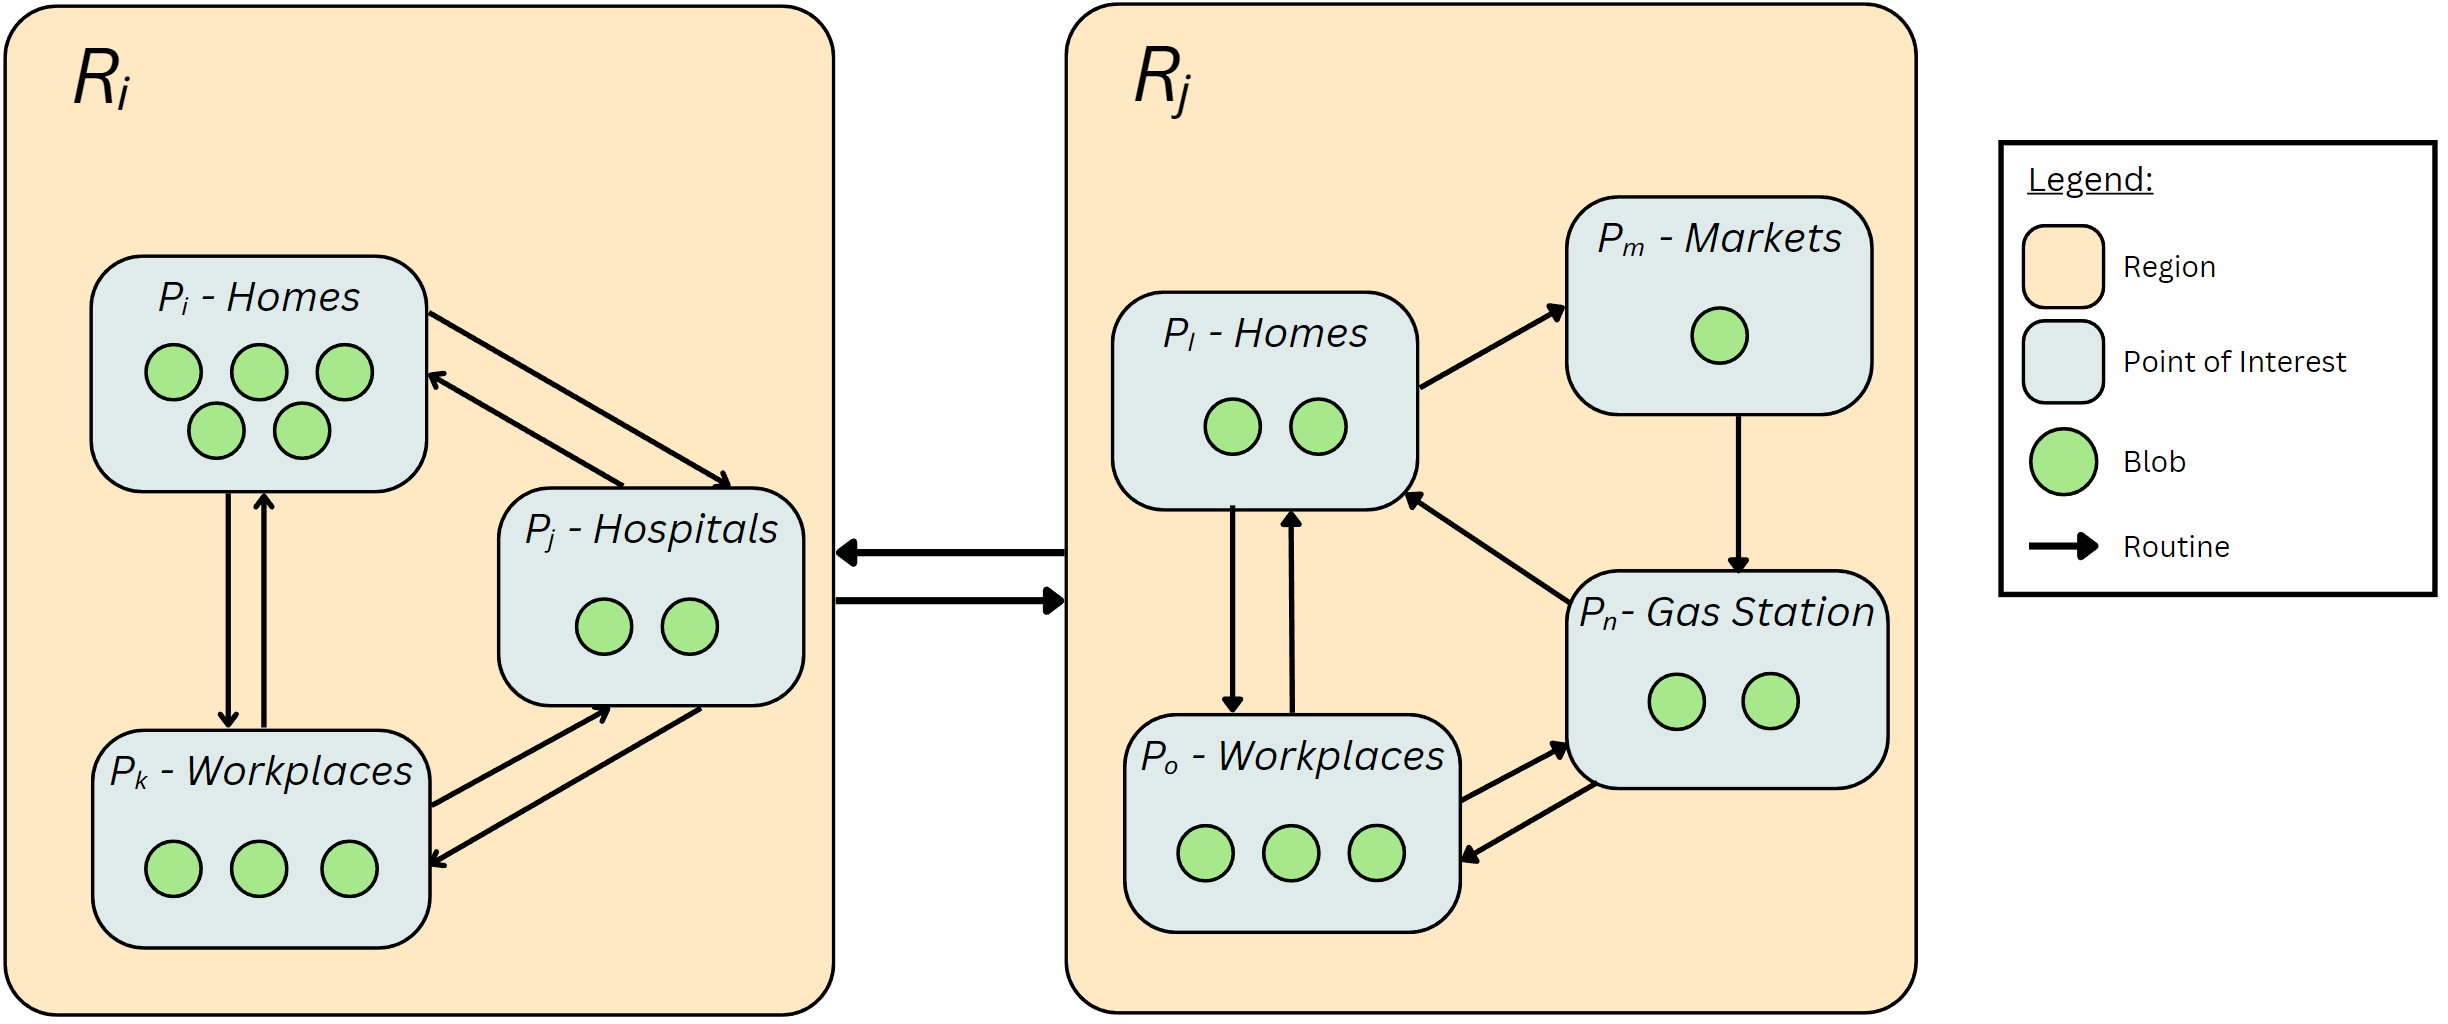
\includegraphics[width=0.98\textwidth]{fig/model/Environment.png}
  \caption{A diagram of a LODUS environment. The figure presents two regions, $R_i$ and $R_j$, containing different points of interest $P$. Each point of interest may contain groups of the population (i.e., blobs), and routines are responsible for moving them in the environment during the simulation.}
  \label{fig1:environment}
\end{figure}

%SO: sobre essa tabela, porque não tem B e RO?
%GA: adicionei
\begin{table}[ht]
\footnotesize
\centering
\caption{Mathematical notation and descriptions of the elements defined in Section~\ref{sec:environment}.}
\label{tbl:notation_env}
\begin{tabularx}{\linewidth}{@{}lcX@{}}
\toprule
\textbf{Element} & \textbf{Notation} & \multicolumn{1}{c}{\textbf{Description}} \\ \midrule
Region & $R$ & Represent areas of physical space in the virtual world that can contain points of interest. A region $R_i$ is defined as a set of $P$. \\ \midrule
\begin{tabular}[c]{@{}l@{}}Point of\\ Interest\end{tabular} & $P$ & Represent locations that the population can occupy as they move during a simulation. A $P_i$ is defined by its type ($\tau_i$), an attribute mapping ($\bm{\alpha}_i$), a collection of population blobs ($\bm{B}_{P_i}$), its local routine ($\bm{Ro}_{P_i}$), its direct disable causes ($\bm{C_i}(t)$), and dependency constraints ($D_i$). \\ \midrule
POI type & $\tau_i$ & Semantic role used to identify locations of the same kind, such as home, work, or school. \\ \midrule
POI attributes & $\bm{\alpha}_i$ & Mapping from named attributes in $K_i$ to their corresponding values in $\mathcal{U}_i$. Values may have different types and may be updated as POI properties change during the simulation. \\ \midrule
Contained blobs & $\bm{B}_{P_i}$ & Collection of population blobs currently located at $P_i$. \\ \midrule
Local routine & $\bm{Ro}_{P_i}$ & Ordered sequence of scheduled actions through which $P_i$ requests population and produces local behavior over time. \\ \midrule
Direct disable causes & $\bm{C_i}(t)$ & Named, independently removable causes that directly prevent $P_i$ from being available at step $t$. \\ \midrule
Dependency constraints & $D_i$ & All-of and minimum-of prerequisite rules used to derive effective availability. \\ %\midrule
%\change{Effective availability} & \change{$e_i(t)$} & %\change{Boolean state obtained from direct causes and the effective states of all prerequisites.} \\ 
\bottomrule
\end{tabularx}
\end{table}

\section{Population}
\label{sec:population}

The population in LODUS is represented by an abstraction of people into blobs $B$, each located at one point of interest at any given simulation step. Blobs describe population groups rather than tracking individuals. A point of interest becoming unavailable does not, by itself, remove or relocate its blobs; any cancellation, waiting, relocation, or redirection of population is performed explicitly by an action according to the policy of the core model or a loaded plugin. 

Formally, a blob is denoted by
\begin{equation}
B=(TP,\bm{Tc},\bm{Sc}),
\label{eq:blob_definition}
\end{equation}
where $TP$ is its total number of individuals, $\bm{Tc}$ is its collection of traceable characteristics, and $\bm{Sc}$ is its collection of sampled characteristics. 

Sampled characteristics ($\bm{Sc}$) represent distributions within the blob. For example, the sampled characteristic \textit{Age} may contain the categories \textit{Child}, \textit{Adult}, and \textit{Elder}, each associated with a number of individuals. Multiple sampled characteristics can jointly describe distributions such as age, schooling level, and employment status. 
%SO: dá um exemplo como fizeste abaixo
%GA: adicionado
For instance, in a blob with $TP=100$, \textit{Age} may contain 20 children, 65 adults, and 15 elders, while \textit{Employment status} may contain 55 employed, 30 unemployed, and 15 student individuals. Each sampled characteristic describes a separate distribution whose category counts sum to $TP$; these marginal distributions do not specify, for example, how many of
the adults are employed.

Traceable characteristics ($\bm{Tc}$) instead store one value for the entire blob. For instance, if \textit{Vaccination status} can be \textit{Vaccinated} or \textit{Unvaccinated}, every individual represented by a particular blob has the same value for that characteristic. 
%SO: será que o traceable lida com personagens com caracteristicas homogeneas e o sampled heetrogeneas?
%GA: a nivel de blob sim, pois a população de uma blob compartilha as mesmas traceable. Mas em nivel de ambiente, as traceables são o que diferenciam as blobs e impedem elas de dar merge.
%The traceable-characteristic schema is simulation-specific. 
% Cola com plugins, talvez remover?
%During initialization, a plugin %SO: Mas, já definimos os plugins???? e essas defs abaixo? sigma... acho que esse texto abaixo está a frente do seu tempo :) TIRAR
%GA: tirado
%may extend it through $E_{\Pi}$ by declaring a characteristic and its default value (Section~\ref{sec:plugins}). The default is applied consistently to the population, after which the characteristic can be read or modified by actions and used as a predicate in population templates.
These characteristics allow us to specify the population in more detail, e.g., elderly people who are currently vaccinated against a given disease or the number of adults who commute to work by bus. Following the previous examples, it becomes possible to track vaccination by age group in the simulation by identifying all blobs $B$ with a \textit{Vaccinated} status and their respective \textit{Age} distributions. Figure~\ref{fig2:blob_diagram} shows the structure of a blob, %SO: quem sabe a blob structure, pois ´bem um diagrama
%GA: ajustado
including its characteristics and associated distributions.

During the simulation, actions generated by the local routine $\bm{Ro}_{P_i}$ may operate on the blobs contained in $P_i$. An action can target a particular population profile, such as children traveling from $P_i$ to a school $P_j$, by applying a population template to the sampled category $Age=Child$.
A population template $T$ specifies which individuals are eligible for an action and the requested quantity. We represent it as

\begin{equation}
T=(T_Q,\bm{T_{Tc}},\bm{T_{Sc}}),
\label{eq:population_template_definition}
\end{equation}

where $T_Q$ is the requested quantity, $\bm{T_{Tc}}$ is an optional set of predicates on traceable characteristics, and $\bm{T_{Sc}}$ is an optional set of predicates on sampled characteristics. Applied to one or more blobs, $T$ filters the eligible population and selects up to $T_Q$ individuals satisfying all declared predicates.


\begin{figure}[ht]
 \centering
  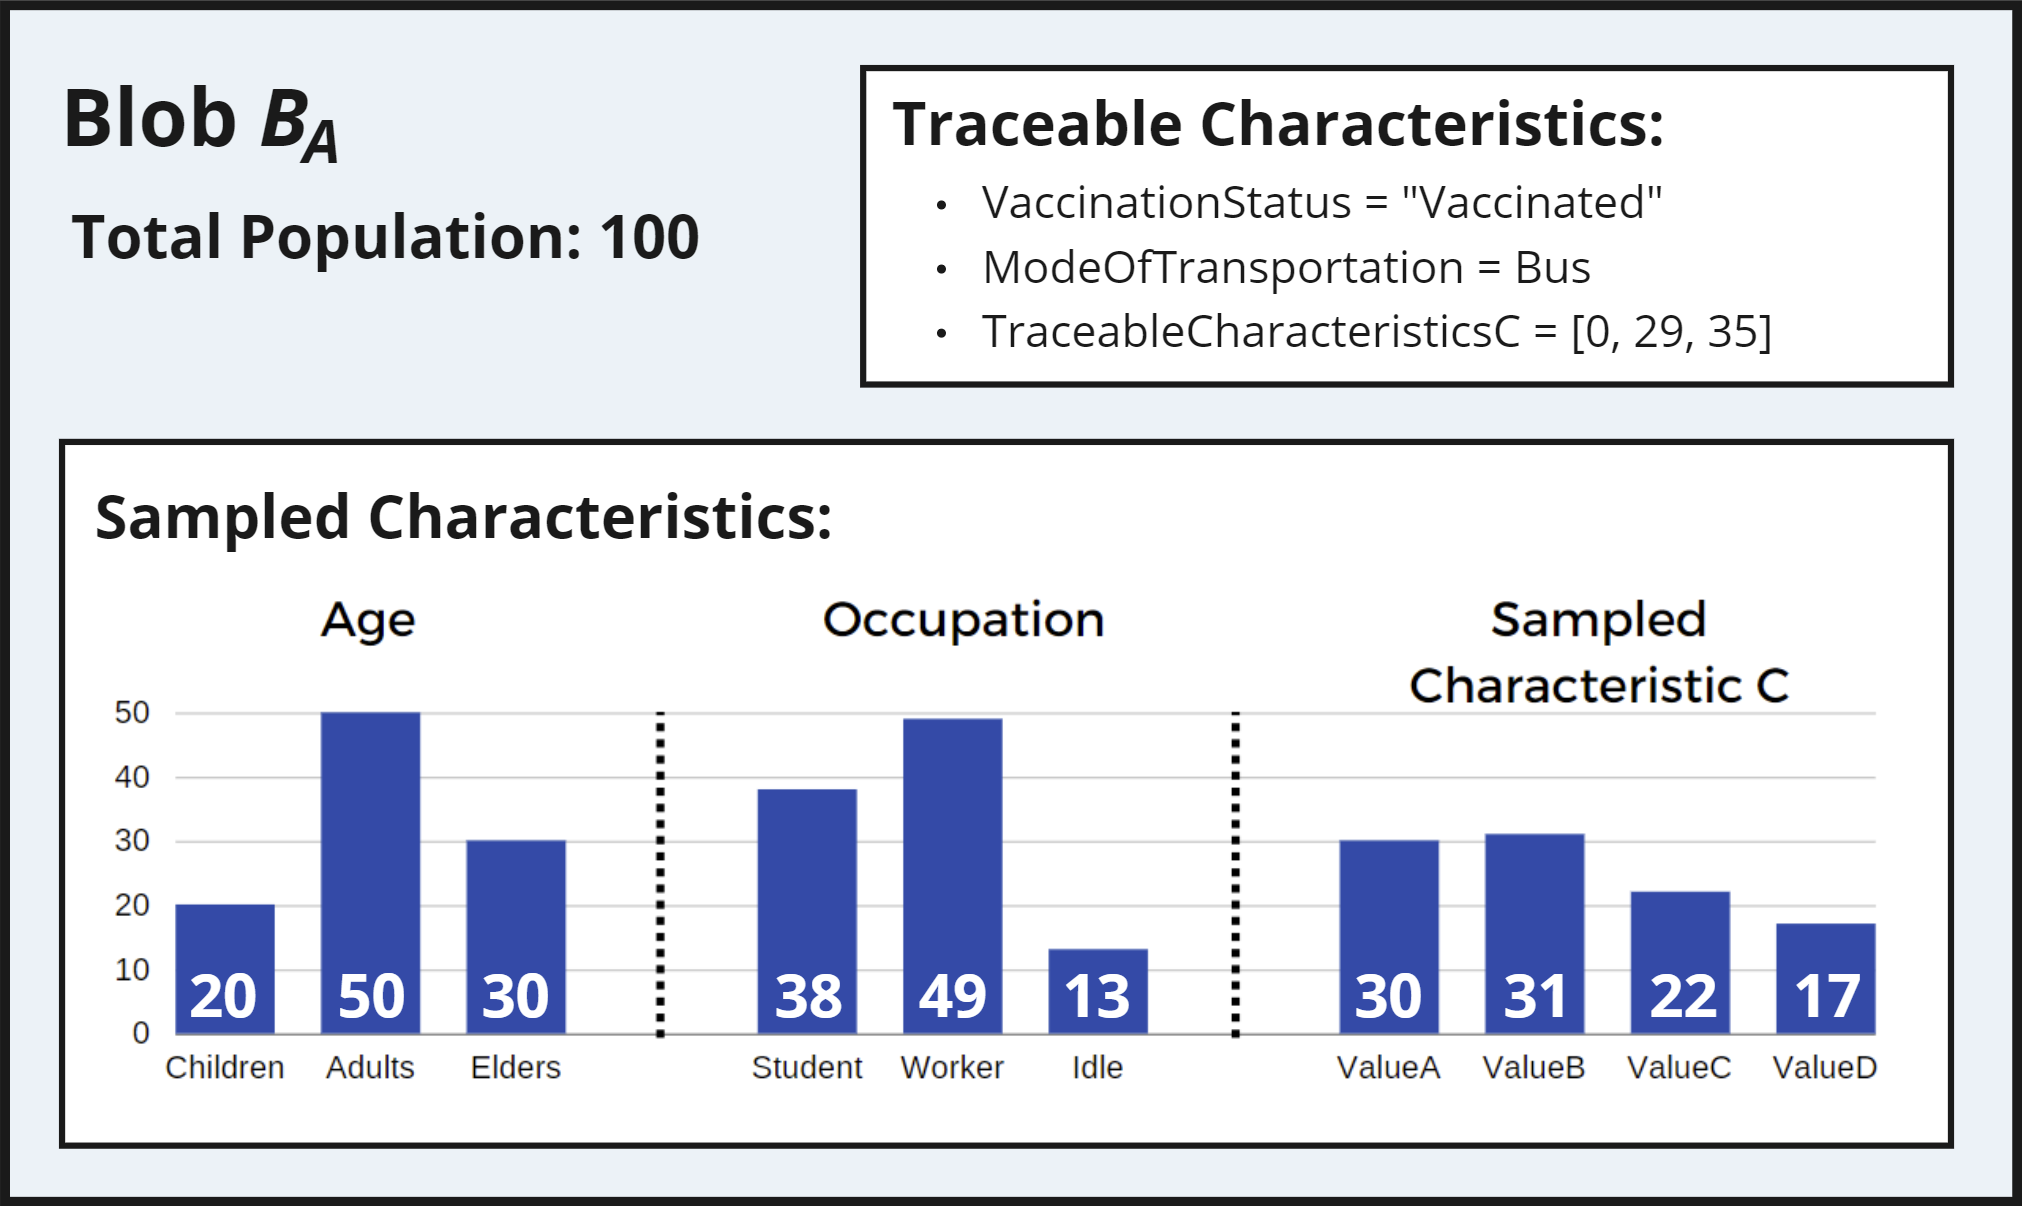
\includegraphics[width=0.9\textwidth]{fig/model/BlobDiagram.png}
  \caption{Structure of a Blob $B_A$ containing 100 people, three traceable characteristics, and three sampled characteristics. Traceable characteristics describe the entire blob population and can have any value type. The distribution of each sampled characteristic sum should be equal to the total population of the blob.} 
  \label{fig2:blob_diagram}
\end{figure}

%SO: abaixo é um exemplo,? então deixa claro
%GA: coloquei um For example,
For example, consider a blob $B_j$ with two sampled characteristics: \textit{i)} \textit{Age}, which includes the possible values \textit{Children}, \textit{Adults}, and \textit{Elders}, and \textit{ii)} \textit{Occupation}, with possible values \textit{Student} and \textit{Worker}. A template $T$ that specifies \textit{Age=Adults} in its collection of sampled characteristics will target only the specified group within $B_j$, in this case, only adults. If the template $T$ does not include a filter for the second sampled characteristic (Occupation), all occupation categories in $B_j$ are affected. The number of affected individuals in categories such as Students and Workers is determined proportionally based on their distribution within $B_j$. For instance, if $B_j$  contains more students than workers, a larger proportion of students will be selected. This process continues until the total number of individuals defined in $T$ is selected or until there are no remaining eligible individuals in $B_j$.

% Splits
When a blob is operated using a population template $T$, it is possible that only a portion of its population may be affected, e.g., a blob $B_i$ that has 75 people and only 20 are selected in $T$. If the operation is to move to another $P$, then such 20 people will create a new blob. This operation generates a split, i.e., the original blob will be separated into two smaller ones. 
In such an example, a template with quantity $T_Q = 20$ selects 20 people from $B_i$ and splits it by creating a new blob $B_j$, which is moved to a different $P$. 
The same occurs when modifying a blob's traceable characteristics ($\bm{Tc}$s). %SO: não é Tsc? 
%GA: não, Tsc são as sampled de um template. Tc são as as traceables de uma blob
For example, another blob $B_k$ has 90 people and a traceable characteristic \textit{InfectionStatus} with value \textit{Healthy}. 20 people are selected, using $T$, to be infected by a disease. The split occurs, and a \textit{InfectionStatus} of $B_l$ (newly created blob) is changed to \textit{Infected}.

% Merge
In addition to split operations, compatible blobs can be merged by combining their total populations $TP$. %SO: TP? Não é TQ? %GA: não, TP é a total population dos blob, TQ é a quantidade pedida por um template
Each sampled characteristic of the resulting blob is obtained by summing the corresponding category counts of the merged blobs. A merge can occur only between blobs in the same point of interest that have equal values for every active traceable characteristic.%, including characteristics introduced by plugins. %SO: tira plugin daqui %GA: done
Consequently, adding a traceable characteristic may also refine the groups that remain distinguishable during merging.
% Figure
Figure~\ref{fig3:blob_operations_with_template} presents a diagram of blobs affected by two templates, resulting in splits and merges. The first scenario, depicted at the top of the figure, demonstrates the relocation of a population. 
The second scenario illustrates changes in traceable characteristics of a population.

%SO: No final desta section citar a tab 1.2 e o apendice
%GA: done
Table~\ref{tbl:notation_pop} summarizes the notation presented in this section. Appendix~\ref{app:input_population} presents an example of the input data required to model the initial population in simulations.

\begin{figure}[ht]
 \centering
  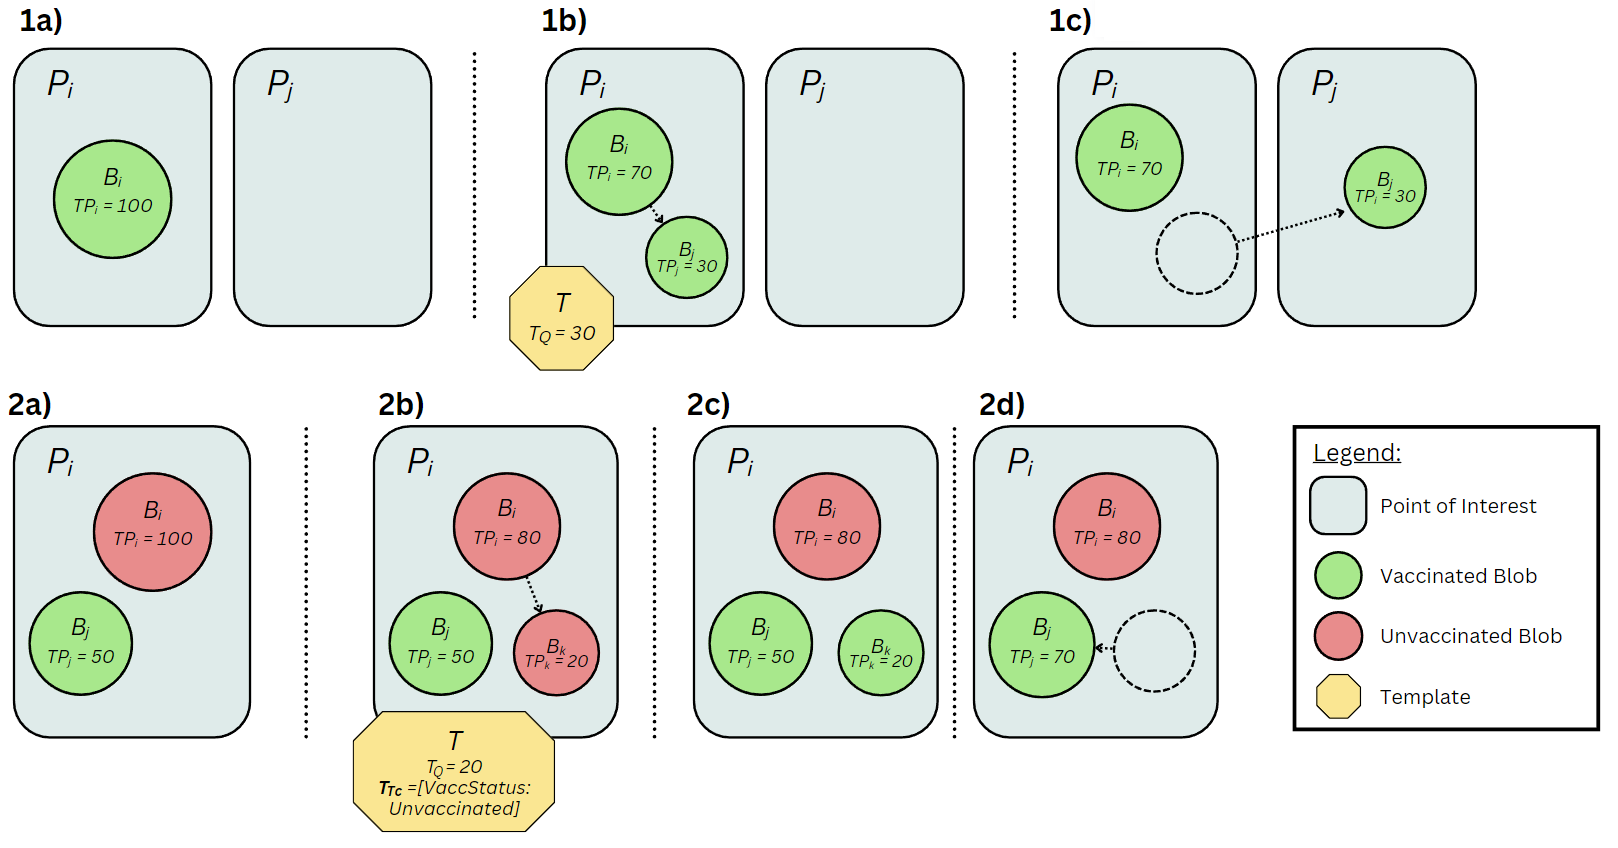
\includegraphics[width=0.99\textwidth]{fig/model/BlobOperations.png}
  \caption{
  Diagram presenting two scenarios of blobs being modified. The first scenario (1) (on the top) shows a population being moved to another location. In 1a, the initial blob $B_i$ has a population of 100. In 1b, a template $T$ selects 30 people, splitting $B_i$ and creating $B_j$. In 1c, $B_j$ is moved to $P_j$. The second scenario (2) shows a population's traceable characteristics changed. In 2a, there are two blobs, $B_i$ containing 100 unvaccinated people (in red), and $B_j$ containing 50 vaccinated people (in green). In 2b, a template $T$ selects 20 unvaccinated people, affecting only $B_i$ and splitting it into $B_k$. In 2c, the traceable characteristic \textit{VaccStatus} of $B_k$ is changed to \textit{Vaccinated}. In 2d, $B_k$ is merged into $B_j$ since they now share the same characteristics and are in the same $P_i$.
  %SO: neste caption achonque podia colocar os nomes das actions MOV e CH
  %GA: Ainda não defini as action até esta hora do texto, mas posso colocar sim
  } 
  \label{fig3:blob_operations_with_template}
\end{figure}

\begin{table}[ht]
\footnotesize
\centering
\caption{Mathematical notation and descriptions of the elements defined in Section~\ref{sec:population}.}
\label{tbl:notation_pop}
\begin{tabularx}{\linewidth}{@{}lcX@{}}
\toprule
\textbf{Element}                                                             & \textbf{Notation} & \multicolumn{1}{c}{\textbf{Description}}                                                                                                                                                                                                                                                                                     \\ \midrule
Blob                                                               & $B$        & Population abstraction $B_i=(TP_i,\bm{Tc}_i,\bm{Sc}_i)$, comprising a total population, traceable characteristics, and sampled characteristics. \\ \midrule
\begin{tabular}[c]{@{}l@{}}Total\\ population\end{tabular} & $TP$ & Number of individuals represented by the blob. \\ \midrule
\begin{tabular}[c]{@{}l@{}}Traceable\\ characteristics\end{tabular} & $\bm{Tc}$ & Collection of identifier--value pairs, each of which has one value shared by the entire blob. \\ \midrule
\begin{tabular}[c]{@{}l@{}}Sampled\\ characteristics\end{tabular} & $\bm{Sc}$ & Collection of categorical distributions over the blob population. For each sampled characteristic, the category counts sum to $TP$. \\ \midrule
\begin{tabular}[c]{@{}l@{}}Population\\ template\end{tabular} & $T$ & Filter $T=(T_Q,\bm{T_{Tc}},\bm{T_{Sc}})$ specifying an eligible population profile and requested quantity for an action. \\ \midrule
\begin{tabular}[c]{@{}l@{}}Requested\\ quantity\end{tabular} & $T_Q$ & Maximum number of eligible individuals requested by the population template. \\ \midrule
\begin{tabular}[c]{@{}l@{}}Traceable-characteristic\\ predicates\end{tabular} & $\bm{T_{Tc}}$ & Optional set of predicates that eligible blobs must satisfy through their traceable characteristics. \\ \midrule
\begin{tabular}[c]{@{}l@{}}Sampled-characteristic\\ predicates\end{tabular} & $\bm{T_{Sc}}$ & Optional set of predicates that select eligible categories from sampled characteristics. \\ \bottomrule
\end{tabularx}
\end{table}

\FloatBarrier


\section{Routines and Actions}
\label{sec:routines}

Behavioral dynamics in LODUS are expressed through routines, which schedule actions at discrete simulation steps. We consider a simulation organized into cycles of fixed length $d$. Let $s\in\mathbb{N}_0$ denote the global simulation-step index. The corresponding step within the current cycle is

\[
t = s \bmod d,
\]

such that $t\in\{0,\ldots,d-1\}$.

A routine is an ordered finite sequence of scheduled actions,

\begin{equation}
Ro=\langle(t_1,A_1),\ldots,(t_n,A_n)\rangle.
\label{eq:routine_definition}
\end{equation}

The ordering is significant when two or more actions share the same cycle step. For each point of interest $P_i$, the local routine $\bm{Ro}_{P_i}$ describes actions requested by that location. The global routine $\bm{GRo}$ has the same structure and schedules actions across the environment rather than being associated with a single point of interest.

Every action retains the common representation

\begin{equation}
A_i=(\kappa_i,T_i,\bm{V}_i),
\label{eq:action_definition}
\end{equation}

%SO: precisas dar um dumping de todas as definições matemáticas e ver se não repetiste nada
where $\kappa_i$ identifies the action type, %SO: N para type é bizarro... 
%GA: mudei para tau, assim como os tipos de pontos de interesse
$T_i$ is a population template, and $\bm{V}_i$ contains the additional parameters required by that action.
Indeed, $\kappa_i$ determines how $T_i$ and $\bm{V}_i$ are interpreted. For population-targeting actions, %SO: como seria N aqui no exemplo? %GA: coloquei um exemplo curto, já que explico em mais detalhe na sequencia
$T_i$ selects the eligible individuals, while an action that does not select a population may ignore an empty template. For example, for a movement action ($\kappa_i=MOV$), $T_i$ may select 20 children and $\bm{V}_i$ specifies the origin and destination points of interest.

In the core model, LODUS provides two built-in action types:
\textit{move population} (MOV), which moves a subset of a blob between points of interest; and \textit{change traceable characteristic} (CH), which modifies the traceable characteristics of a subset of a blob.
A MOV action expects its parameter vector $\bm{V}$ to specify an origin and a destination point of interest. For example, the local routine of $P_i$ may include the pair $(t = 15, A)$, where $A = (MOV, T_i, \bm{V}_i)$, with $T_i=(T_Q=20, T_{Tc}=\emptyset, T_{Sc}=\{Age=Child\})$, and $\bm{V}_i$ encoding $P_i$ as origin and $P_j$ as destination. At cycle step $t = 15$, this action selects 20 children from the blobs at $P_i$, splits them into a new blob, and moves that blob to $P_j$.

A CH action expects $\bm{V}$ to contain the name of a traceable characteristic and its new value. For instance, the local routine of $P_j$ may include $(t = 25, A')$, with $A' = (CH, T_j, \bm{V}_j)$, where $T_j=(T_Q=20, T_{Tc}=\{Status=Unvaccinated\}, T_{Sc}=\emptyset)$, and $\bm{V}_j$ encodes the update ``Status = Vaccinated''. At cycle step $t=25$, this action selects 20 unvaccinated individuals from the blobs at $P_j$, splits them into a new blob, and changes the traceable characteristic Status of that blob to Vaccinated. Figure~\ref{fig3:blob_operations_with_template} illustrates both the movement and characteristic-change scenarios.


% Global routines and Queueing
The same action representation is used by the global routine $\bm{GRo}$. For example, MOV or CH entries in $\bm{GRo}$ may schedule effects across all points of interest at cycle step $t$, enabling global phenomena such as random walks or disease spread. These actions share a scheduling step but are consumed sequentially, not simultaneously. 


To produce repeating temporal behavior, the simulation iterates over cycle steps $t=0,\ldots,d-1$. At cycle step $t$, actions are processed in the following phases:
%SO: eu tirei o s lá de cima que estava confuso. Ver se tem que colocar de volta, mas deixando mais claro. Aqui abaixo fala de plugin
%GA: aqui deve bastar, tirei a parte de plugins de novo
\begin{enumerate}
    \item actions scheduled for cycle step $t$ by $\bm{GRo}$ and each $\bm{Ro}_{P_i}$ are collected;
    \item the collected actions are applied sequentially in their defined order; and
    \item after all actions have been applied, compatible blobs at each point of interest are merged.
\end{enumerate}

%SO: honestamente não vi razão no parágrafo abaixo. Só repetição... podes resumir talvez
%GA: resumido
Before each population-targeting action is applied, its template is evaluated against the current simulation state. Consequently, later actions account for any splits, movements, or characteristic changes produced by preceding actions at the same cycle step.
Figure~\ref{fig:simulation_diagram} illustrates the simulation behavior over one simulation step, and Appendix~\ref{app:simulator} presents an example of the overall simulation control flow.


%SO: mudar a figura, tirar hook, handler e plugin

\begin{figure}[ht]
 \centering
  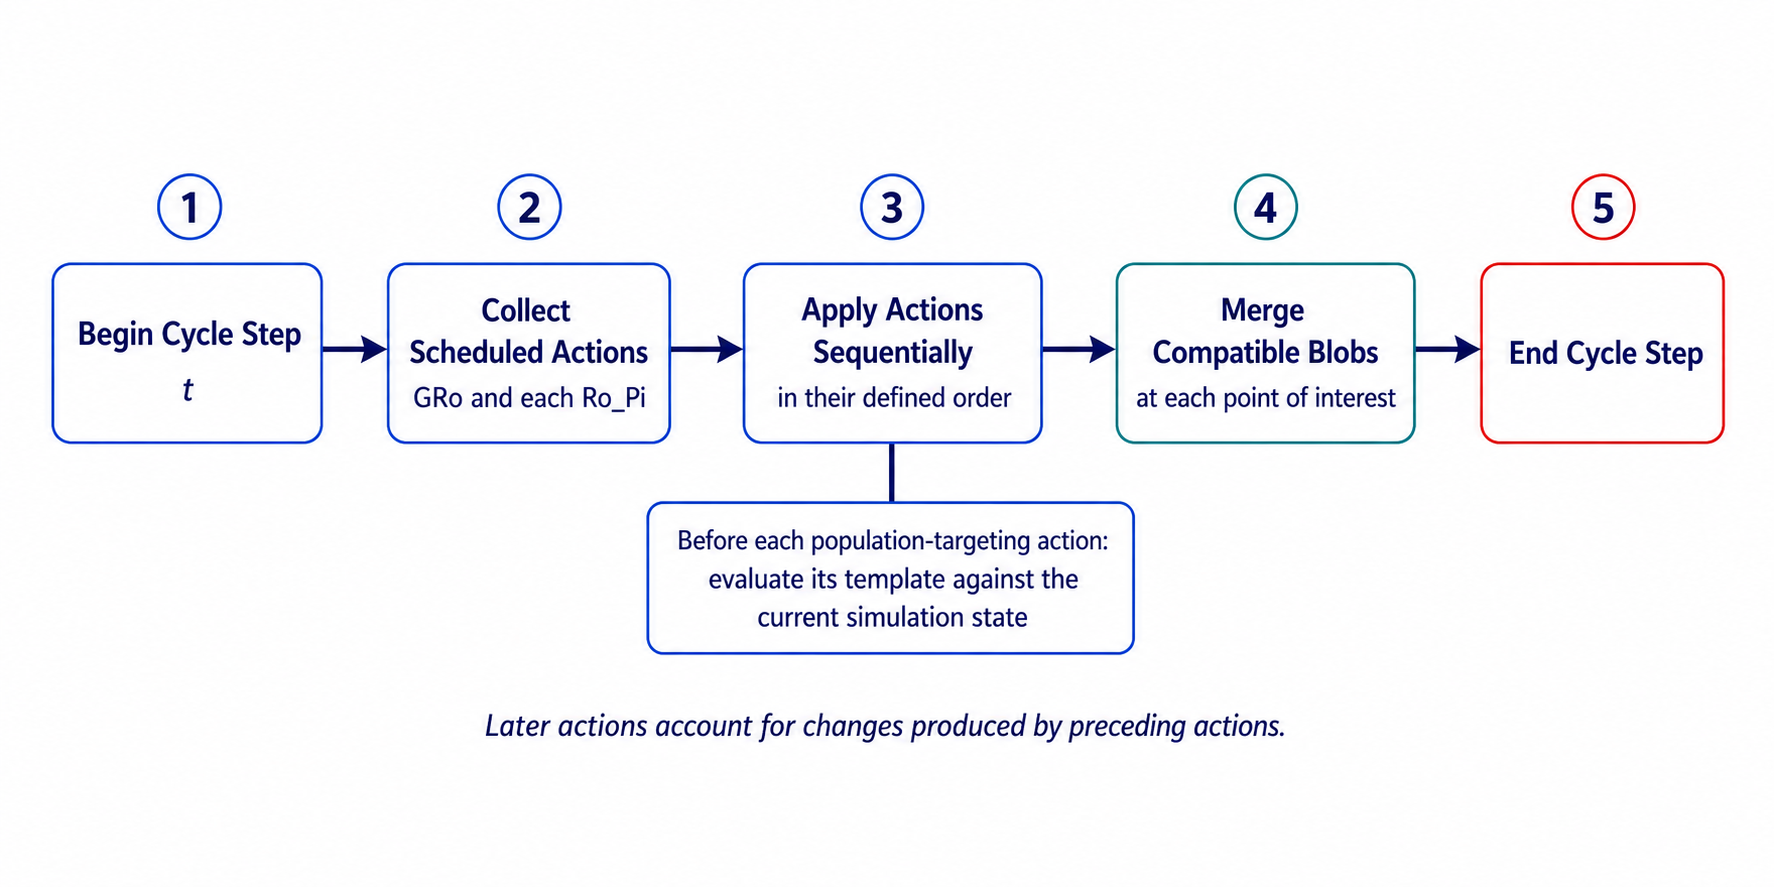
\includegraphics[width=0.99\textwidth]{fig/model/SimulationBehaviorDiagramMethodology.png}
  \caption{Execution flow of one LODUS cycle step. Actions scheduled by the global and local routines are collected and applied sequentially in their defined order. Each action observes the state produced by preceding actions. After all scheduled actions have been applied, compatible blobs at each point of interest are merged.}
  \label{fig:simulation_diagram}
\end{figure}


%GA: deixei o link para o apendice aqui
Table~\ref{tbl:notation_rout} summarizes thee notation presented in this section. Appendix~\ref{app:input_routine} provides an example of the input data used to encode local and global routines.

%SO: trouxe a tabela mais para perto
%GA: coloquei mais para o final pois inclui notações de ações e rotinas
\begin{table}[ht]
\footnotesize
\centering
\caption{Mathematical notation and descriptions of the elements defined in Section~\ref{sec:routines}.}
\label{tbl:notation_rout}
\begin{tabularx}{\linewidth}{@{}lcX@{}}
\toprule
\textbf{Element} & \textbf{Notation} & \multicolumn{1}{c}{\textbf{Description}} \\ \midrule
\begin{tabular}[c]{@{}l@{}}Cycle\\ length\end{tabular} & $d$ & Number of discrete simulation steps in each cycle. \\ \midrule
\begin{tabular}[c]{@{}l@{}}Cycle\\ step\end{tabular} & $t$ & Step within the current cycle, where $0\leq t<d$. \\ \midrule
Routine & $\bm{Ro}$ & Ordered finite sequence $\langle(t_1,A_1),\ldots,(t_n,A_n)\rangle$ of scheduled actions. \\ \midrule
\begin{tabular}[c]{@{}l@{}}Routine\\ entry\end{tabular} & $(t_i,A_i)$ & Action $A_i$ scheduled for cycle step $t_i$. \\ \midrule
\begin{tabular}[c]{@{}l@{}}Local\\ routine\end{tabular} & $\bm{Ro}_{P_i}$ & Ordered routine associated with $P_i$, describing actions requested by that point of interest. \\ \midrule
\begin{tabular}[c]{@{}l@{}}Global\\ routine\end{tabular} & $\bm{GRo}$ & Ordered routine used to schedule actions across the environment rather than at one point of interest. \\ \midrule
Action & $A_i$ & Action $A_i=(\kappa_i,T_i,\bm{V}_i)$, comprising a type, a population template, and additional parameter values. \\ \midrule
\begin{tabular}[c]{@{}l@{}}Action\\ type\end{tabular} & $\kappa_i$ & Identifier that determines how $T_i$ and $\bm{V}_i$ are interpreted. \\ \midrule
\begin{tabular}[c]{@{}l@{}}Population\\ template\end{tabular} & $T_i$ & Template that selects the population eligible for action $A_i$; defined in Section~\ref{sec:population}. \\ \midrule
\begin{tabular}[c]{@{}l@{}}Additional action\\ parameters\end{tabular} & $\bm{V}_i$ & Values required by action type $\kappa_i$, such as origin and destination POIs for MOV. \\ %\midrule
%\begin{tabular}[c]{@{}l@{}}Core action\\ types\end{tabular} & $MOV, CH$ & Move population and change traceable characteristic, respectively. \\ 
\bottomrule
\end{tabularx}
\end{table}

%SO: só a partir daqui pode haver plugin
%GA: deixo este trecho?
%\change{The core action types establish the population-transition semantics shared by all LodusPop simulations. Domain-specific actions, routines, state updates, and observations are introduced through plugins, described in the following section.}


\FloatBarrier
%SO: re-escrevi todo. validar.
\section{Extension Mechanism}
\label{sec:extension_mechanism}

The core model presented in the previous sections defines the structures and behaviors shared by all LODUS simulations: an environment composed of regions and points of interest, a population represented by blobs and population templates, and routines and actions that modify the simulation state over time.

Different application domains, however, may require additional information or behaviors. For example, an epidemic simulation may need to distinguish susceptible and infected populations, a flood simulation may need to associate water-level information with points of interest, and a health-service simulation may require capacity and treatment rules. These elements should not be part of every LODUS simulation.

To support these domain-specific requirements, LODUS adopts an extension mechanism implemented through \emph{plugins}. A plugin augments the core model rather than replacing it. In other words, plugins reuse the same regions, points of interest, blobs, population templates, routines, and actions defined by the core model, while adding only the information and behavior required by a particular simulation. A plugin may extend the core model in one or more of the following ways:

\begin{itemize}
    \item \textbf{Population extensions}, by introducing additional traceable characteristics and their default values. For example, a plugin may add an infection status, vaccination level, or treatment state to the existing blob representation;

    \item \textbf{Environment extensions}, by defining additional point of interest, new attributes or by modifying their state. For example, a flood plugin may interpret a water-level threshold stored in a point of interest and make that location unavailable when the threshold is exceeded;

    \item \textbf{Behavior extensions}, by contributing routines or defining additional action types. These actions follow the same representation $A_i=(\kappa_i,T_i,\bm{V}_i)$ introduced in Section~\ref{sec:routines}, and therefore use the same population-selection and execution mechanisms as the core actions; and

    \item \textbf{Simulation extensions}, by performing domain-specific updates or observations at defined moments of the simulation, such as updating an environmental condition, recording service demand, or collecting experiment-specific outputs.
\end{itemize}

Thus, plugins provide a controlled way of adapting LODUS to different application domains without changing the fundamental abstractions of the model. A simulation is obtained by combining the core model with the set of plugins required by the scenario and by supplying their corresponding parameters.

For consistency with the experimental chapters, the contribution of a plugin $\Pi$ is described using the components summarized in Table~\ref{tbl:notation_plugins} and defined in Equation~\ref{eq:extension}:

\begin{equation}
%\[
\Pi =
\left(
\theta_{\Pi},
E_{\Pi},
R_{\Pi},
F_{\Pi},
H_{\Pi}
\right),
%\]
\label{eq:extension}
\end{equation}


where:

\begin{itemize}
    \item $\theta_{\Pi}$ contains the parameters that configure the plugin for a particular experiment;

    \item $E_\Pi$ represents extensions to the core model, such as additional traceable characteristics or point-of-interest attributes;

    \item $R_{\Pi}$ represents routines or scheduled actions contributed by the plugin;

    \item $F_{\Pi}$ represents additional action types and their execution semantics; and

    \item $H_{\Pi}$ represents optional simulation-step updates, observations, data access, or output recording associated with the plugin.
\end{itemize}

These components are only descriptive categories for organizing plugin contributions; a plugin does not need to provide all of them. 
In many cases, only one or two extensions are required. For instance, a movement-restriction plugin may only provide a parameter and expose its value during the simulation, whereas an epidemic plugin may add a population characteristic and define an action that changes this characteristic.

An important aspect of this design is that domain-specific behavior remains separate from the state represented by the core model. A point of interest, for example, stores its attributes and availability state, but the consequences of becoming unavailable are intentionally left to the application-specific plugins. Depending on the application, a plugin may cancel the corresponding demand, redirect it to another location, place it in a queue, or generate a new action. 
Similarly, blobs retain the same representation regardless of whether they are being used to model mobility, infection, evacuation, or access to health services.

This separation allows the same LODUS model to support different simulation domains while preserving a common representation of population and environment.
The experimental scenarios presented in Chapter~\ref{chapter:experimental_results} illustrate this mechanism by progressively extending the core model with mobility, epidemic, environmental-disruption, shelter, and health-service
behaviors.

\begin{comment}
\section{Extension Mechanism} %SO: mudei o nome
\label{sec:plugins}

%SO: re-escrevi. Valide
The core model presented in the previous sections defines the structures and execution rules common to all LODUS simulations, thereby representing their intrinsic behavior. However, different application domains may require additional behaviors or domain-specific actions. To support such extensions, LODUS adopts an extension mechanism that augments, rather than replaces, the core model by using software components as plugins. So, a simulation is configured by selecting the appropriate set of plugins and their associated parameters. Depending on its purpose, a plugin may introduce new traceable characteristics and their default values, define point-of-interest attributes, contribute routines, define additional action types, trigger or generate actions, provide domain-specific data, or record simulation outputs.

%The core model, as presented in the last sections, represents the structures and execution rules shared by all simulations, i.e., the innate behavior of all simulation in LODUS. However, depending on the simulation to be designer, other actions or behaviors can be necessary. To acomplish with that, we propose the plugins which aimjs to provide the behavior required for a particular application domain. Plugins extend rather than replace points of interest, blobs, population templates, routines, and actions. A new simulationt selects a set of plugins and supplies their parameters. Depending on its role, a plugin may add traceable characteristics and their defaults, define conventions for point-of-interest attributes, contribute routines, register new action types, invoke or emit other actions, expose data services, or record outputs.

Let $\mathcal{S}(s)$ denote the complete simulation state at simulation step $s$, 
%SO: ver se s index não é t
including points of interest, blobs, routines, availability states, and action registries. 
A plugin $\Pi$ is defined through the extension contract

% Notação sugerida por IA com base na implementação de plugins
\begin{equation}
\Pi=\left(\bm{\theta}_{\Pi},E_{\Pi},\mathcal{R}_{\Pi},
\mathcal{F}_{\Pi},\mathcal{H}_{\Pi}\right),
\label{eq:plugin_definition}
\end{equation}

where:
\begin{itemize}
    \item $\bm{\theta}_{\Pi}$ is a finite key--value mapping of parameters read from the experiment configuration;
    %SO: não entendi o que é esse parãmtro, para que serve
    \item $E_{\Pi}$ contains optional additions to the model vocabulary, including declarations and defaults for traceable characteristics and point-of-interest attribute conventions; %SO: mas porque delta? por causa do additions? isso é viagem do gpt
    \item $\mathcal{R}_{\Pi}$ is an optional finite collection of local-routine, global-routine, start-of-step, or end-of-step action contributions;
    %SO: deveria ser um vetor então?
    \item $\mathcal{F}_{\Pi}=\{(N,f_N)\}$ is an optional registry associating action-type identifiers with the handlers that consume them; and
    %SO: tu já não tens action type e "handlers"?
    \item $\mathcal{H}_{\Pi}$ defines the optional extension points associated with the simulation lifecycle, time-step execution, data access, observation, and output recording.
    %\item $\mathcal{H}_{\Pi}$ contains optional lifecycle, time-step,
    data-access, observation, and logging hooks.
\end{itemize}

Any component may be empty, and a plugin need only use the extension points required by its role. %The notation consequently covers action, routine, logger, and data plugins without requiring each plugin to implement every mechanism.
At load time, the simulator reads $\bm{\theta}_{\Pi}$, applies the declarations in $E_{\Pi}$, incorporates $\mathcal{R}_{\Pi}$, registers $\mathcal{F}_{\Pi}$, and activates $\mathcal{H}_{\Pi}$. 
During execution, each registered pair $(N,f_N)$ associates an action identifier $N$ with the handler that consumes actions of that type. 
Plugin actions retain the common action structure $A=(N,T,\bm{V})$, so their handlers receive the same population template and additional values used by core actions. At a high level, a handler is described as

\begin{equation}
f_N:\bigl(\mathcal{S}(s),T,\bm{V},t,s;\bm{\theta}_{\Pi}\bigr)
\longmapsto
\bigl(\mathcal{S}'(s),\langle A_1,\ldots,A_\ell\rangle\bigr).
\label{eq:plugin_action_handler}
\end{equation}

% Ações simples e complexax
A primitive handler applies its transition directly to $\mathcal{S}$ and may return an empty action sequence. A composite handler may instead return core or plugin-defined actions, which are consumed through the same $A=(N,T,\bm{V})$ contract. This makes calls to other actions explicit while preserving population-template selection and sequential execution.

The lifecycle and observation hooks in $\mathcal{H}_{\Pi}$ allow a plugin to update the simulation at step boundaries, expose data to other plugins, record state, and release its resources. 
% Abaixo, plugins que dependem de outros plugins
A loaded set of plugins $\mathbb{P}=\{\Pi_1,\ldots,\Pi_r\}$ is valid when its action identifiers and schema declarations are compatible and all plugin requirements are present.
%Dependencies between plugins must be stated by the experiment; for example, a mobility plugin may require an action type provided by a population-gathering plugin. 
%Appendix~\ref{app:plugin} illustrates the implementation of such an extension.

The same definition provides a reporting template for the experimental chapters:

\begin{equation}
\Pi_x=(\bm{\theta}_x,\Delta\Sigma_x,\mathcal{R}_x,
\mathcal{F}_x,\mathcal{H}_x).
\label{eq:experiment_plugin_template}
\end{equation}

An experiment need only describe the nonempty components and the scenario values of $\bm{\theta}_x$. For example, a dialysis plugin can state its capacity and service parameters in $\bm{\theta}_x$, patient-state characteristics in $\Delta\Sigma_x$, scheduled requests in $\mathcal{R}_x$, and service handlers and update hooks in $\mathcal{F}_x$ and $\mathcal{H}_x$.

% Diferença de informações de POIs vs Plugins acessando e modificando o comportamento base
Point-of-interest state and plugin behavior remain distinct. The tuple $P_i$ defines where location data are stored and how effective availability is derived. The tuple $\Pi$ defines the experiment-specific rules that read or modify that state and determine the population response. 
For example, a flood plugin may compare a forcing value with a threshold in $\bm{\alpha}_i$ and add a cause to $C_i(t)$. The dependency constraints $D_i$ then propagate effective unavailability, after which a mobility or service plugin decides whether the resulting demand is canceled, queued, or redirected. Service capacities, queues, flood thresholds, patient stays, destination substitution, and commute lifecycles consequently remain explicit plugin policies rather than universal fields of every blob or point of interest.


\begin{table}[ht]
\footnotesize
\centering
\caption{Mathematical notation and descriptions of the plugin extension contract.}
\label{tbl:notation_plugins}
\begin{tabularx}{\linewidth}{@{}lcX@{}}
\toprule
\textbf{Element} & \textbf{Notation} & \multicolumn{1}{c}{\textbf{Description}} \\ \midrule
Plugin & $\Pi$ & Extension contract $(\bm{\theta}_{\Pi},E_{\Pi},\mathcal{R}_{\Pi},\mathcal{F}_{\Pi},\mathcal{H}_{\Pi})$. \\ \midrule
Configuration & $\bm{\theta}_{\Pi}$ & Experiment-supplied parameter mapping. \\ \midrule
Schema additions & $E_{\Pi}$ & Population characteristics, defaults, and POI-attribute conventions introduced by the plugin. \\ \midrule
Routine contributions & $\mathcal{R}_{\Pi}$ & Local, global, start-of-step, or end-of-step actions contributed by the plugin. \\ \midrule
Action registry & $\mathcal{F}_{\Pi}$ & Pairs $(N,f_N)$ associating action identifiers with consuming handlers. \\ \midrule
Hooks and services & $\mathcal{H}_{\Pi}$ & Lifecycle, time-step, data-access, observation, and logging interfaces. \\ \bottomrule
\end{tabularx}
\end{table}


\begin{table}[ht]
\footnotesize
\centering
\caption{Mathematical notation describing the contributions of a LodusPop plugin.}
\label{tbl:notation_plugins}
\begin{tabularx}{\linewidth}{@{}lcX@{}}
\toprule
\textbf{Element} & \textbf{Notation} & \multicolumn{1}{c}{\textbf{Description}} \\ \midrule

Plugin &
$\Pi$ &
Plugin contribution described by $(\bm{\theta}_{\Pi},E_{\Pi},\mathcal{R}_{\Pi},\mathcal{F}_{\Pi},\mathcal{H}_{\Pi})$. \\ \midrule

Configuration &
$\bm{\theta}_{\Pi}$ &
Experiment-specific parameters used to configure the plugin. \\ \midrule

Model extensions &
$E_{\Pi}$ &
Additional traceable characteristics, point-of-interest attributes, or other domain-specific elements introduced into the core model. \\ \midrule

Routine contributions &
$\mathcal{R}_{\Pi}$ &
Additional routines contributed by the plugin. \\ \midrule

Action extensions &
$\mathcal{F}_{\Pi}$ &
Additional action types together with their execution semantics. \\ \midrule

Simulation extensions &
$\mathcal{H}_{\Pi}$ &
Simulation-step updates, observations, data access, or output recording contributed by the plugin. \\

\bottomrule
\end{tabularx}
\end{table}
\end{comment}

\begin{table}[ht]
\footnotesize
\centering
\caption{Mathematical notation describing the contributions of a LODUS plugin.}
\label{tbl:notation_plugins}
\begin{tabularx}{\linewidth}{@{}lcX@{}}
\toprule
\textbf{Element} & \textbf{Notation} & \multicolumn{1}{c}{\textbf{Description}} \\ 
\midrule

Plugin &
$\Pi$ &
Plugin contribution described by $(\theta_{\Pi},E_{\Pi},R_{\Pi},F_{\Pi},H_{\Pi})$. \\ 
\midrule

Configuration &
$\theta_{\Pi}$ &
Experiment-specific parameters used to configure the plugin. \\ 
\midrule

Model extensions &
$E_{\Pi}$ &
Additional traceable characteristics, point-of-interest attributes, or other domain-specific elements introduced into the core model. \\ 
\midrule

Routine contributions &
$R_{\Pi}$ &
Additional routines or scheduled actions contributed by the plugin. \\ 
\midrule

Action extensions &
$F_{\Pi}$ &
Additional action types together with their execution semantics. \\ 
\midrule

Simulation extensions &
$H_{\Pi}$ &
Simulation-step updates, observations, data access, or output recording associated with the plugin. \\

\bottomrule
\end{tabularx}
\end{table}

%\FloatBarrier

% ---------------------------------------------------------------------------
% Definições alternativas para plugins (sugestões de IA)
% ALTERNATIVE PLUGIN DEFINITION 2 (compact transition-operator view)
% This option treats a configured plugin as one operator over state and pending
% actions. It is compact, but hides which extension mechanisms an experiment uses.
% \[
% \Pi_{\bm{\theta}}:\mathcal{S}\times A^{*}\longrightarrow
% \mathcal{S}\times A^{*}.
% \]
% The operator may transform state, consume actions, and emit actions. Setup,
% routine injection, logging, and schema changes would require separate prose.

% ALTERNATIVE PLUGIN DEFINITION 3 (base-model delta view)
% This option defines a plugin by the changes it contributes to a base simulator.
% It emphasizes composition, but is less convenient for parameters and stateful
% hooks in an experimental specification.
% \[
% \Pi=(\Delta\Sigma,\Delta Ro,\Delta F,\Delta H),
% \qquad M_{\Pi}=M_0\oplus\Pi.
% \]
% Here \Delta\Sigma extends the schema, \Delta Ro extends routines, \Delta F
% extends the action registry, and \Delta H extends lifecycle and observation
% hooks. Parameters would be supplied separately as \Pi_{\bm{\theta}}.
% ---------------------------------------------------------------------------
